\documentclass{article}
\usepackage{enumitem}
\usepackage{fancyhdr}
\usepackage{listings}
\usepackage{graphicx}
\usepackage{hyperref}
\usepackage{supertabular}

\usepackage{xcolor}
\usepackage{array}
\usepackage{colortbl}
\usepackage{easy-todo}
\usepackage{tikz}
\usepackage{titlesec}
\usetikzlibrary{arrows.meta, positioning}
\definecolor{nextAssesment}{RGB}{34, 139, 34} % Define a custom color
\definecolor{completedAssessment}{RGB}{200, 200, 240}
\definecolor{otherAssessment}{RGB}{250,100,100}
\definecolor{FE}{RGB}{34, 139, 34}
\definecolor{CA}{RGB}{255, 165, 0}

\titleformat{\section}
  {\huge\bfseries}
  {\thesection}
  {1em}
  {}
  \titleformat{\subsection}
  {\Large\bfseries}
  {\thesubsection}
  {1em}
  {}
% for exercise 
%% Change this for title information 
\newcommand\ExTitle{\ Course Outline and Essential Information}
\author{Mair\'ead Meagher, SETU}

\newcommand\fullExTitle{Functional Programming
\\ \ExTitle \\Semester 2 - '24-'25 }
\newcommand\footerExTitle{\ExTitle -\ Functional Programming }

\pagestyle{fancy}
\fancyhead{} % clear all header fields
\renewcommand{\headrulewidth}{0pt} % no line in header area
\fancyfoot{} % clear all footer fields
\fancyfoot[LE,RO]{\thepage}           % page number in "outer" position of footer line
\fancyfoot[RE,LO]{\footerExTitle} % other info in "inner" position of footer line

%\usepackage[mathrm,colour,cntbysection]{czt}

\begin{document}
\begin{Huge}
	\begin{center}
	\fullExTitle \\
    \vspace{.1cm}
    Mair\'ead Meagher, SETU.
    \end{center}
\end{Huge}
\begin{center}
    \begin{tabular}{|c |  c | }
 
    \hline 
    \includegraphics[width=1.5in]{img/RGB.png} &          \includegraphics[width=1.5in]{img/mairead-avatar.jpeg} \\ 

   
    %  \rowcolor{red!60}
    %  \textbf{Assignment}& Vet Appl  & Vet Appl  & Prog assign  & Prog assign\\  
    %  \rowcolor{red!60}
    
        & Mair\'ead Meagher  \\  
       & \href{mailto:mmeagher@wit.ie}{mairead.meagher@setu.ie} \\

    \hline
    \multicolumn{2}{|c|}{Department of Computing and Mathematics} \\
     \hline

  
    \end{tabular}
\end{center}

\pagebreak

\tableofcontents
\pagebreak
\section{Module Name}   
\Large{ \textbf{Functional Programming} }\\
This is the year 4, semester 2 running of this module in South East Technological University. 
\section{Lecturer}
\Large{ \textbf{Mair\'ead Meagher,}} \\
Lecturer in Department of Computing and Mathematics, \\
School of Science and Computing,
South East Technological University.

\section{How to reach me}
\begin{itemize}
    \item The quickest way to reach me is via Slack (please join the Functional Programming  Slack workspace  
    \href{https://join.slack.com/t/functionalpro-k8d2114/shared_invite/zt-3ntbgw544-Q3NZOYkgXaDMSs3WW80yzg}{here} ).  
    \textbf{I will be using  this  as the main form of communication for this running of the module. }

    \item You can also reach me via email:\\ \href{mailto:mairead.meagher@setu.ie}{mairead.meagher@setu.ie}. 
    \item I am available during work hours from Monday to Friday, 9am to 5pm. You can \textbf{Slack me (preferable)} or email me  outside 
    of these hours and I will reply as soon as I can, 
but always within three days.(If this does not happen, assume your contact has gone into spam etc. and please re-contact me.) 
When emailing me, please indicate what module you are taking as well as the nature of your query in the 
subject line.

\end{itemize}

\section{Learning Approaches}
\subsection{Learning Technologies}
We will be using 
\begin{itemize}
        \item \textbf{tutors} - This static website will hold all the notes, labs and links to video See Figure \ref{tutors}.
    This site has the  course published as far as we have covered at any time so you can navigate in whatever way suits you.  
    There is a facility to produce a local version (snapshot) at any time. 
    This may be useful if there are network issues during the year. If you would like such a version at any time, just ask me. 
    These obviously will not contain any subsequent  updates so use with caution. 
\begin{figure}[h]
    \centering
    \includegraphics[width=.5\textwidth]{img/tutors.png}
    \caption{Example of tutors website}
    \label{tutors}
\end{figure}
\pagebreak
\item \textbf{Slack} - our main communication platform. We will use Slack for:
\begin{itemize}
    \item \textbf{Announcements} - I will post announcements on Slack from time to time.
    \item \textbf{Questions} - you can ask questions on Slack and I will answer them as soon as I can. If the 
    question is relevant to the whole class, ask it in a general channel and I will post the answer in a thread.
    If the question is relevant to just you, ask it in your private channel and I will answer it there. 
    \item \textbf{Discussion} - you can discuss topics with your classmates on Slack.    
    \item \textbf{Threads} - please use threads to keep the channels tidy. It takes a little getting used to, but it is worth it!
    \item \textbf{channels} - please use the appropriate channels for your questions and discussions. I may create new channels as needed.
\end{itemize}
\item \textbf{Moodle} - our learning management system. 
We use Moodle for 
\begin{itemize} 
    \item  Uploading assessments 
    \item  Each week you will be given a todo list of materials/labs/exercises 
    that should be  completed before the next week.
    \item Quizzes - there will  be quizzes on Moodle during the semester.
    \item Announcements - I will post announcements on Moodle from time to time (but mainly on Slack).
\end{itemize}


\subsection{Technologies used in the module}
\item \textbf{IDE} - We need to use an IDE (Integrated Development Environment) to write and manage Haskell code.
I suggest the VSCode IDE with the Haskell extension. You are welcome to use whichever IDE you prefer, but I will be using \textbf{VSCode} in the labs and examples. I will be using VSCode in the labs and examples. 
\item \textbf{GitHub Classroom} - We will be using GitHub Classroom to manage the programming assignment. 
This will allow me to monitor your progress on the assignment and give you feedback as you go along.
\item \textbf{GHCI} - The Glasgow Haskell Compiler interactive environment. This is the interactive environment for Haskell. 
We will be using this in labs and exercises.
\item \textbf{Stack} - The Haskell build tool. We will be using Stack to manage Haskell projects.
\end{itemize}

\subsection{Structure of lectures/ labs}
Your timetable structure is: 
\begin{itemize}
\item 14 weeks (12 weeks of tuition)
\item 4 hours per week.
\end{itemize}
During each of these contact hours, we will have (interchangeably) either/both:
\begin{itemize}
    \item Lectures 
    \item Labs practising techniques we have seen in lectures
    \item Working through/reviewing exercises sheets. 
\end{itemize}
Because of this fluid structure, \textbf{I will ask that you bring your laptops to all classes}.
If any of you have a problem with this, contact me as a matter of urgency. 

The module is broken down into 12-14 topics. These topics are curated on tutors. 
Each topic will have associated with it: 
\begin{itemize}
    \item Lecture/s 
    \item Labs - either practical work using Haskell or exercises sheets. 
\end{itemize}
  




\section{Module objectives /\ Learning outcomes}
On completion of this module students should be able to: 
\begin{enumerate}
    \item  Construct simple and more complex programs in Haskell;
    \item  Construct basic constructs of Haskell;
    \item  Use tools to help build Haskell projects, notably GHCI and Stack;
    \item  Improve the scope of programs by using Haskell libraries;
    \item  Write programs to solve problems in specific domains, e.g. parsing;
    \item  Write suitable tests for Haskell programs, including property-based tests; 
\end{enumerate}

\section{Assessment Breakdown} 
This module has a final exam at the end of the semester and continuous assessment during the semester. The 
continuous assessment in this module is made up of one \textit{formative} and three \textit{summative} assignments.

\begin{figure}[htbp]
\centering
\resizebox{0.9\textwidth}{!}{
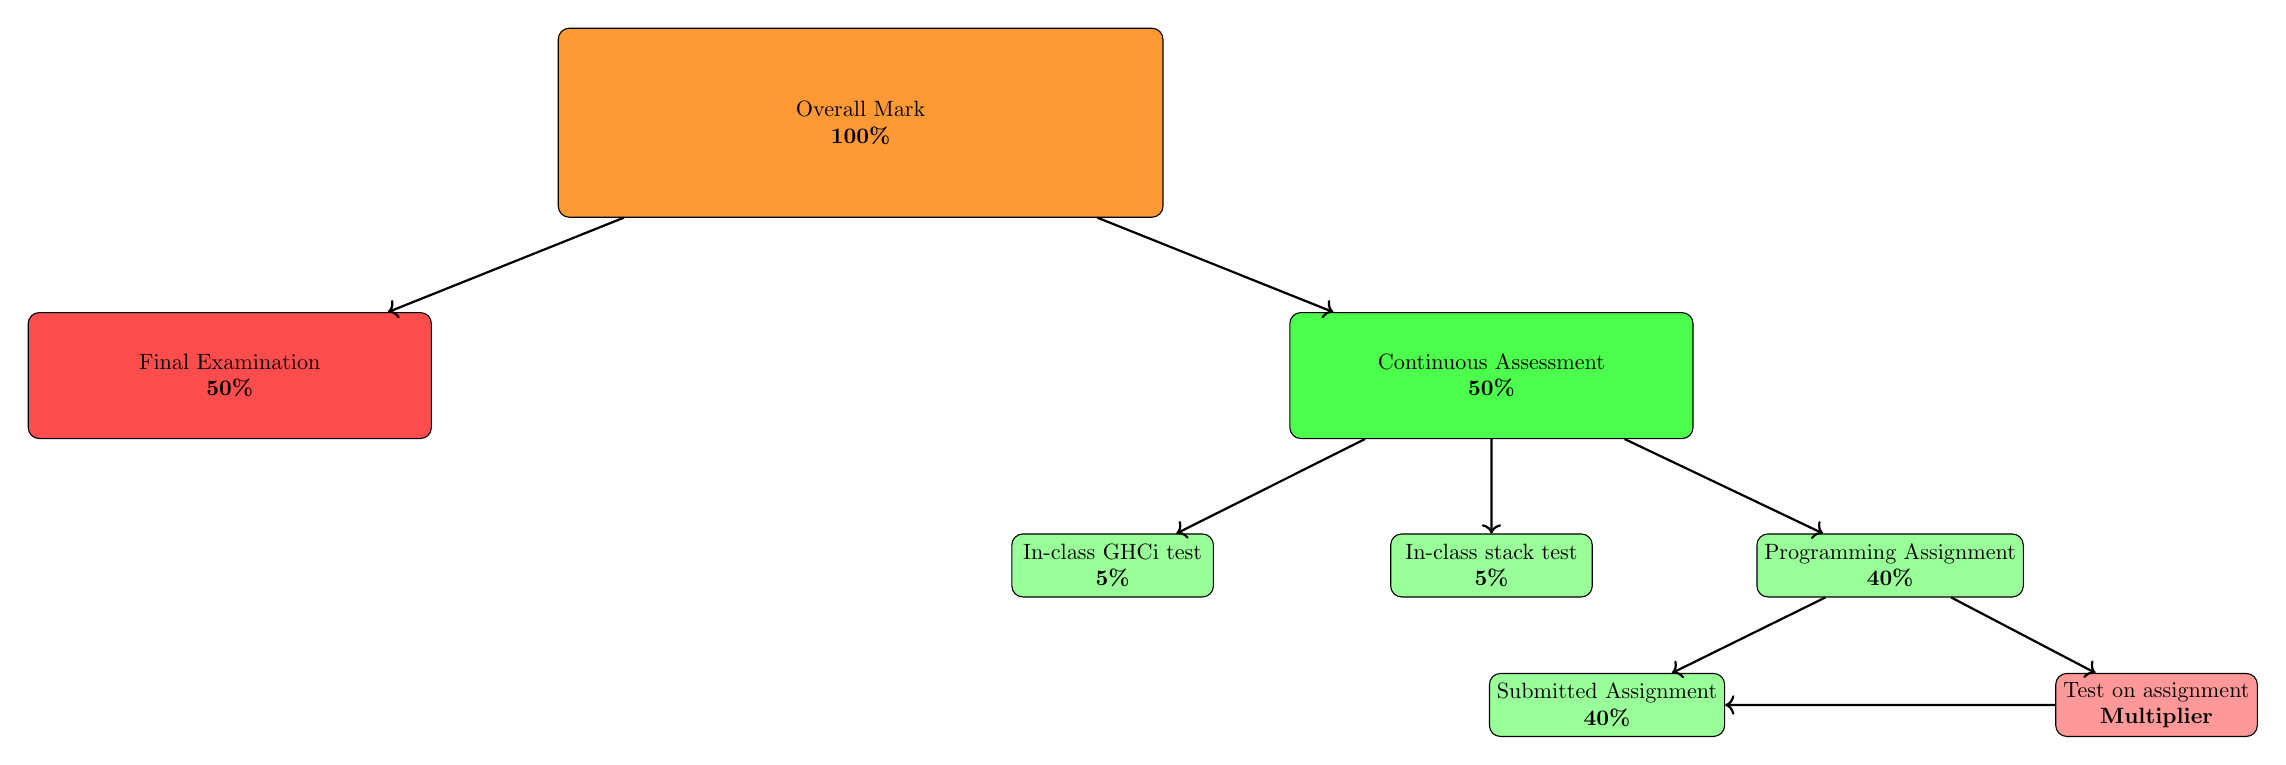
\begin{tikzpicture}[
  scale=0.8,
  transform shape,
  box/.style={
    rectangle,
    draw,
    rounded corners,
    align=center,
    minimum width=3.2cm,
    minimum height=1cm
  },
  bigbox/.style={
    rectangle,
    draw,
    rounded corners,
    align=center,
    minimum width=9.6cm,
    minimum height=3cm
  },
  medbox/.style={
    rectangle,
    draw,
    rounded corners,
    align=center,
    minimum width=6.4cm,
    minimum height=2cm
  },
  arrow/.style={->, thick},
  over/.style={bigbox, fill=orange!80},
  exam/.style={medbox, fill=red!70},
  ca/.style={medbox, fill=green!70},
  caitem/.style={box, fill=green!40},
  multiplier/.style={box, fill=red!40}
]

\node[over] (overall) {Overall Mark\\\textbf{100\%}};

\node[exam, below left=1.5cm and 2cm of overall] (exam)
{Final Examination\\\textbf{50\%}};

\node[ca, below right=1.5cm and 2cm of overall] (ca)
{Continuous Assessment\\\textbf{50\%}};

\node[caitem, below left=1.5cm and 1.2cm of ca] (ic1)
{In-class GHCi test\\\textbf{5\%}};

\node[caitem, below=1.5cm of ca] (ic2)
{In-class stack test\\\textbf{5\%}};

\node[caitem, below right=1.5cm and 1cm of ca] (proga)
{Programming Assignment\\\textbf{40\%}};

\node[caitem, below left=1.2cm and 0.5cm of proga] (subm)
{Submitted Assignment\\\textbf{40\%}};

\node[multiplier, below right=1.2cm and 0.5cm of proga] (stest)
{Test on assignment\\\textbf{Multiplier}};

\draw[arrow] (overall) -- (exam);
\draw[arrow] (overall) -- (ca);
\draw[arrow] (ca) -- (ic1);
\draw[arrow] (ca) -- (ic2);
\draw[arrow] (ca) -- (proga);
\draw[arrow] (proga) -- (subm);
\draw[arrow] (proga) -- (stest);
\draw[arrow] (stest) -- (subm);

\end{tikzpicture}

}
\caption{Breakdown of Formative Assessment and Final Exam}
  \label{fig:assessment-structure}
\end{figure}
The asessment in this module is made up of continuous assessment during the module and a Final Exam at the end of the semester. 
The schedule for the continuous assessment is seen at Figure \ref{ass-exel-sheet} - Assignment Schedule. 
\begin{enumerate}
    \item \textbf{Written Final Exam} (50\%) This will be a written final exam. 
    \item  \textbf{Continuous Assessment} (50\%) broken into 
    \begin{itemize}
        \item In class lab test - 5\% - starting using GHCI – this is to ensure that all students are competent in using GHCI and writing small Haskell programs. It includes fixing syntax errors, e.g. filling in missing type declarations in simple functions.
        \item In class lab test - 5\% - using Stack – a simple program using the Stack structure.
        \item  0\% formative programming assignment (phase 1 of programming assignment).
        \item  40\% programming assignment (including the written test and\/or interview).
    \end{itemize}
   
\end{enumerate}
\begin{center}
    \begin{figure}[h]
        \centering
        \includegraphics[width=.5\textwidth]{img/sched-excel.png}
        \caption{Schedule of assessment}
        \label{ass-exel-sheet}
    \end{figure}
\end{center}
% \begin{table}[h]
% \begin{center}
%     \begin{tabular}{|>{\columncolor{blue!10}}c | c | c | c |  c |}
%         \rowcolor{completedAssessment}
%         \cellcolor{completedAssessment} COMPLETED &\cellcolor{completedAssessment} COMPLETED& \cellcolor{nextAssesment}NEXT DUE&\cellcolor{otherAssessment}TO COME &\cellcolor{otherAssessment}TO COME\\ 
%         \hline

%         \cellcolor{completedAssessment} GHCI lab test  &\cellcolor{completedAssessment}lab test Stack &\cellcolor{nextAssesment}  Form Assign & \cellcolor{otherAssessment}Prog Assign & \cellcolor{otherAssessment}Final Exam \\  
    
%     \hline
%     \rowcolor{completedAssessment}
%      5\% &\cellcolor{completedAssessment} 5\% &\cellcolor{nextAssesment} 0\% & \cellcolor{otherAssessment}40\% & \cellcolor{otherAssessment}50\% \\ 
%     \hline
%     \rowcolor{completedAssessment}
%     \rowcolor{completedAssessment}Week 3 & \cellcolor{completedAssessment}Week 7 &\cellcolor{nextAssesment} Week 9 & \cellcolor{otherAssessment}Week 12 & \cellcolor{otherAssessment}Week 13/14\\ 
%      \hline
%      \rowcolor{completedAssessment}
%      11:15 & \cellcolor{completedAssessment}11:15 & \cellcolor{nextAssesment}18:00 & \cellcolor{otherAssessment}18:00, Sunday & \cellcolor{otherAssessment}tbc \\ 
    
%      \rowcolor{completedAssessment}
   
%      \rowcolor{completedAssessment}6th Feb & \cellcolor{completedAssessment} 13th March & \cellcolor{nextAssesment}27nd March & \cellcolor{otherAssessment}5th May & \cellcolor{otherAssessment}  \\ 
%      \hline
    
%      \hline
    
   
     
%      \rowcolor{completedAssessment}
%      \cellcolor{completedAssessment} &\cellcolor{completedAssessment} & \cellcolor{nextAssesment} &\cellcolor{otherAssessment}Interviews &\cellcolor{otherAssessment}\\ 
%     \rowcolor{completedAssessment}
%     \cellcolor{completedAssessment} &\cellcolor{completedAssessment} & \cellcolor{nextAssesment} &\cellcolor{otherAssessment}Monday 6th May  &\cellcolor{otherAssessment}\\ 

%      \hline
  
%     \end{tabular}
%     \caption{Assessment Schedule}
%     \label{tab:ass-schedule}   

     
% \end{center}
% \end{table}




The CA is rolled out in the above order so that you, the student, can steadily build up marks throughout the semester. 

For all the continuous assessment submitted during the module, you will get your marks back as soon as is possible, but usually within a week. 
If you are wondering why you got a particular mark, \textbf{always} ask me. My marking schemes are very comprehensive and I am happy to go through the breakdowns with you. 
I don't give this comprehensive feedback by default to speed up the return of the marks but am happy to engage about them later. 

For the in-class lab tests, I will give you sample lab tests so that you know the nature of the tests beforehand. 

For the programming assignment, a marking scheme will be published with the specification of the assignment. I will ask you to use GitHub Classroom so that I can monitor your regularity of work on the assignment.
The assignment will be broken down into phases, and the first phase will be formative. This is to ensure that you are on the right track. 
The formative assignment is worth 0\% of your module, but by completing it, you will be able to get feedback on your progress 
and should help you to build your confidence for the remainder of the assignment.

As always, be sure that you are aware of the marking scheme. 
If there are marks going for a particular part, and you haven't attempted that part, there is nothing I can do. \begin{quote}\textbf{Always make it easy for the examiner to give you marks!}\end{quote}

If you wish to seek an extension for an assignment, you must do so in sufficient time (i.e. not on the day of submission, and not 
when the submission date has passed) and must provide a valid reason for seeking the extension. 




\section{Academic Integrity}
The School of Science and Computing  at South East Technological University are  committed to maintaining the highest standards of academic integrity. 
Academic misconduct, including, but not limited to, cheating may result in a mark of zero for the assignment as well as disciplinary action.
Additional sanctions may by imposed depending on the case. You are responsible for ensuring that you do not get involved in cheating of any kind. 
 
\begin{subsection}{Use of AI Bots in assessment}{use-of-ai-bots}
    The use of AI bots is widespread and becoming part of a productive development environment. 
    However, there are a number of issues around the use of AI bots in assessment. The blind use of AI bots can lead to error-prone code, and a lack of understanding thereof. 
    This lack of understanding of the code can lead to a lack of reflection and a lack of understanding of the code. The lack of reflection and lack of understanding
    of the code makes it difficult to fix issues that arise. The more you understand the fundamentals of coding, the better you will be able to use AI bots effectively and productively.
    You are then able to use the code suggested by the AI bot, modify it, and improve it rather than copying it blindly and 'hoping for the best'. The aim of this module is to ensure 
    that you understand the fundamentals of functional programming in Haskell so that you can be productive developers with or without AI bots whilst   
    always having the full control of the code you produce.
    Therefore, the following rules will apply to the programming assignment in this module with regard to the use of AI bots:
\begin{itemize}
    \item You are allowed to use AI bots for development of code. 
    \item You must reference the use of AI bots in your submission. 
    \item You must reflect on the use of AI bots in your submission. (more pointers will be given at the time of assignment specification).
    \item You must be able to explain the code that you submit in a written test and\/or interview.
    \item You must be able to trace how you developed a section/s of code, including how and why you changed/improved code that was originally suggested by the AI bot.
    \item You will have a post-submission in-class test on the assignment. This will test your understanding of the code that you submitted. 
    A mark will be given for this test and this markused as a multiplier for your assignment mark. If the mark is < 50\% I will interview you on the assignment. 
    I also reserve the right to interview you on the assignment if I have any concerns about the authenticity of the work submitted or, indeed, if I chose to do so randomly. 
\end{itemize}
 
\end{subsection}

I  will always encourage you to work in collaboration with your fellow classmates. 
But please be careful not to cross the line between collaboration and using someone else's work. 


Please do not be tempted to go down  this route. I will help you in any way I can during the semester. 
But if you take this route, I \textbf{will} take formal action. 
That is not a position either of us wish to be in. 
It is too risky and the penalty can affect your academic future. 

\pagebreak
\section{Important note about engagement in the module  and time management}
 Part of active engagement  for any module involves a degree of time management. You will be given exercises and labs to do, sometimes beetween class times.
 These will not be graded but, by engaging in these tasks at the time, you will be in a better position to 
 understand the next part of the module. We will approach the module in a step-by-step manner, so opting out at any part will make it more difficult for you to keep up. 
 This is where time management will come in - you need to be careful to ensure that you keep a balance between modules. 
 
 Always ask questions, either in class or after class.  One way to help to stay engaged is to ask questions if you don't understand what is going on. 
 Remember, when you are asking questions:
 \begin{itemize}
    \item Just the process of formulating and asking a question means that you have learned something. 
    \item If you cannot understand, in most cases, you are not the only one. 
    \item Asking questions means that the pace of the lecture/ labs will suit you better - I will always keep going if there are no questions! 
 \end{itemize}

 \section{Netiquette and Decorum}
 We will use Slack mainy as our forum for online communiication. Please follow a number of guidelines in your use of Slack: 
 \begin{itemize}
\item Always remember this is a public forum. Be careful and respectful in what you say. No need to be too formal, but please no text speak
or bad language. 
 \item If a question or comment is something that is specific to your situation, please use DM, not a public channel;
 \item If you are replying to a comment/question on a public channel, please use the 'Reply' to stay in the thread. 
 This leads to a much tidier and more useful channel;
 \item Please put up your picture up on your profile. I haven't seen you for a while, and then there were masks involved!
 
 \end{itemize}
 
 \subsection{Netiquette}
 The word netiquette is a combination of ’net’ (from internet) and ’etiquette’. It means respecting other users’ views and displaying 
 courtesy when posting  questions or comments online. Here are some guidelines to follow when communicating online, e.g. Slack or email:
 \begin{itemize}
    \item Remember that there is a human being on the other end of your communication
    \item Treat that human being with respect
    \item Do not post a message that you would not be willing to communicate in a face to face environment.
    \item Keep it courteous
    \item Be kind and professional:  Online communication comes with a level of anonymity that doesn’t exist when you’re talking to someone face-to-face. 
    Sometimes this leads people to behave rudely when they disagree with one another. Online students probably don’t have the complete anonymity that comes with using a screen name, but you could still fall prey to treating someone poorly because of the distance between screens. Make a point to be kind and respectful in your comments—even if you disagree with someone.
    \item Extend your good nature online: The digital world is an increasingly important part of our lives. We should be our best selves there too. The manners our parents taught us apply everywhere.
    \item Promote healthy discussions: 
    To get the most out of online forums, a useful netiquette guideline is to promote healthy discussion. You can help your online community by posing questions, sharing experiences, providing positive feedback, asking follow-up questions, and referring to information sources. Being a positive contributor is better than being a critic, troll or other negative force.
    \item Ignore inflammatory comments by trolls
    It's generally best to ignore trolls. These are internet users who try to bait other users into a reaction. Trolls might be honest in what they're saying, or they could be sarcastic or deliberately dishonest. You can tell a troll by the inflammatory nature of their statements. They want to stir up negative emotions and responses.
    \item  Respect others as equals:
    Show a little respect and humility online. Think – that 'idiot' who wrote the opinion you completely disagree with is a human being. They have feelings and experiences. They may believe passionately in what they're saying. And they may actually be right.
    Even if you're feeling dismissive or knowledgeable or whatever, inject respect into your writing. That's just being fair to others.
    \item You're here to learn and contribute, not dictate: 
    While we all like to think that our opinion matters, you'll gain more from internet forums by approaching them as a learner.
    When everyone is trying to express their view rather than hearing from others, forums become noisy, crowded with posts, and disjointed. 
    A more polite and effective path is to adopt a listening mode. Read posts carefully, ask questions, and write something only if it offers value to the discussion.
    \item Read first
    Take some time to read through each of the previous discussion post responses before writing your own response. Remember, discussions can move fairly quickly so it’s important to absorb all of the information before crafting your reply. Building upon a classmate’s thought or attempting to add something new to the conversation will show your instructor you’ve been paying attention.
    \item Remember, your words are permanent: Be careful with what you post online. Once it's out there, you may not be able to get it back.
    \item Make your point in a nice way:
    Write in a way to get the kind of reaction you want. A little thoughtfulness, strategy and netiquette can go a long way in online discussions.
    Your first draft of an online post is unlikely to be your best. Are you disagreeing with someone in a flippant way? Have you misinterpreted what they really meant? Will you put people off with the tone of your text.
    \item Pause before you post:
    It's worth taking a moment to reflect before hitting the send button.
    When you're using a computer, you're normally clicking, and scrolling and typing all over the place. Most things are done quickly. But one time when it's important to slow down is when you're about to post something online for all the world to see. Pause and reflect for a second. Are you truly comfortable with what you're sending?
    \item Respect the opinion of your classmates: 
    If you feel the need to disagree, do so respectfully and acknowledge the valid points in your classmate's argument. If you reply to a question from a classmate, make sure your answer is accurate!
    \item Forgive and Forget
    If you’re offended by something another student says online, keep in mind that you may have misunderstood their intentions. Give them the benefit of the doubt.
 \end{itemize}

 \section{Engagement in the module  and time management}
 Part of active engagement  for any module involves a degree of time management.
 As part of this module, I will be asking you to complete tutorial sheets, labs and quizzes between class times. 
 These will not be graded but, by engaging in these tasks at the time, you will be in a better position to
 understand the next part of the module. We will approach the module in a step-by-step manner, 
 so opting out at any part will make it more difficult for you to keep up.
 This is where time management will come in - you need to be careful to ensure that you keep a balance between modules.
 You should be organising your time \textbf{ruthlessly} especially this semester. Ensure that you are planning your time 
 so that you can keep (somewhat!) in control of your workload. You \textbf{must} be proactive in this regard and use some planner, 
 be it digital or paper based, to ensure that you are keeping on top of your workload.

 Always ask questions, either in class or during labs.  One way to help to stay engaged is to ask questions if you don't understand what is going on.
 Remember, when you are asking questions:
 \begin{enumerate}
    \item Just the process of asking a question means that you have learned something.
    \item If you cannot understand, in most cases, you are not the only one.
    \item Asking questions means that the pace of the lecture/ labs will suit you better - We will always keep going if there are no questions!
 \end{enumerate}
\section{Final words}
I am looking forward to working with you all this semester. 
If you have any questions, please do not hesitate to ask me.
\end{document}